\documentclass[14pt,aspectratio=169]{beamer}
%\documentclass[notes=only,aspectratio=149]{beamer}   % only notes

\usetheme{wasp}

\usepackage[utf8]{inputenc}
\usepackage[british]{babel}
\usepackage{pbox}

\title{Presentation Title}

\author{Authors}
\subtitle{Subtitle}
\date{\today}

\newcommand{\twocols}[4]{%
\noblocktitles%
\begin{columns}[t]%
\column{#1\textwidth}\begin{block}{}#3\end{block}%
\column{#2\textwidth}\begin{block}{}#4\end{block}%
\end{columns}%
}

\newcommand{\twocolstitled}[6]{%
\blocktitles%
\begin{columns}[t]%
\column{#1\textwidth}\begin{block}{#3}#5\end{block}%
\column{#2\textwidth}\begin{block}{#4}#6\end{block}%
\end{columns}%
}

\newcommand{\threecols}[6]{%
\noblocktitles%
\begin{columns}[t]%
\column{#1\textwidth}\begin{block}{}#4\end{block}%
\column{#2\textwidth}\begin{block}{}#5\end{block}%
\column{#3\textwidth}\begin{block}{}#6\end{block}%
\end{columns}%
}

\newcommand{\threecolstitled}[9]{%
\blocktitles%
\begin{columns}[t]%
\column{#1\textwidth}\begin{block}{#4}#7\end{block}%
\column{#2\textwidth}\begin{block}{#5}#8\end{block}%
\column{#3\textwidth}\begin{block}{#6}#9\end{block}%
\end{columns}%
}

\begin{document}

\titleframe

\section{A section}
\setbeamercovered{transparent}

\setlength{\fboxsep}{0pt}
\begin{frame}{Example Slide}
\framesubtitle{With a picture from the WASP 2016 kick-off}
\twocols{0.4}{0.6}{
	This page
	\begin{itemize}
    	\item Has an itemized list
		\item Split in two columns
		\item The other column is wider and contains the image
	\end{itemize}
}{\fcolorbox{waspgrey}{white}{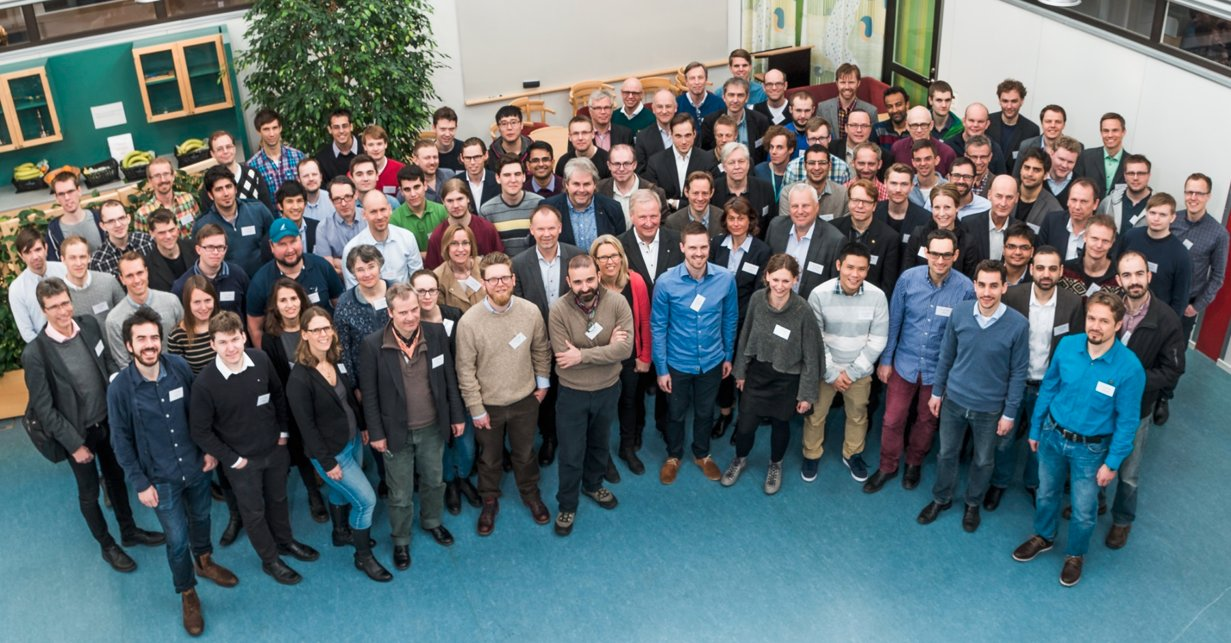
\includegraphics[width=\textwidth]{waspko.jpg}}}
\end{frame}
\note{This will show if you set the option 'notes=only' in the document class}

\begin{frame}{Another Example Slide}
\framesubtitle{}
\begin{itemize}
	\item With another itemized list.
	\item This slide does not have a subtitle.
\end{itemize}
\end{frame}
\note{Another note.}


\begin{frame}{Grayed Out Items}
\framesubtitle{Which generates several slides}
\begin{itemize}
\item<2-> The items in this list are initially greyed out
\item<3-> But as you press space etc they will light up
\item<4-> To emphasize the current topic
\end{itemize}
\end{frame}
\note{And of course, the page notes.}


\begin{frame}{An example with three titled columns}
\framesubtitle{A slight gray around images make a huge difference}
\threecolstitled{0.28}{0.28}{0.28}{Lectures}{Work}{Social Activities}
{\fcolorbox{waspgrey}{white}{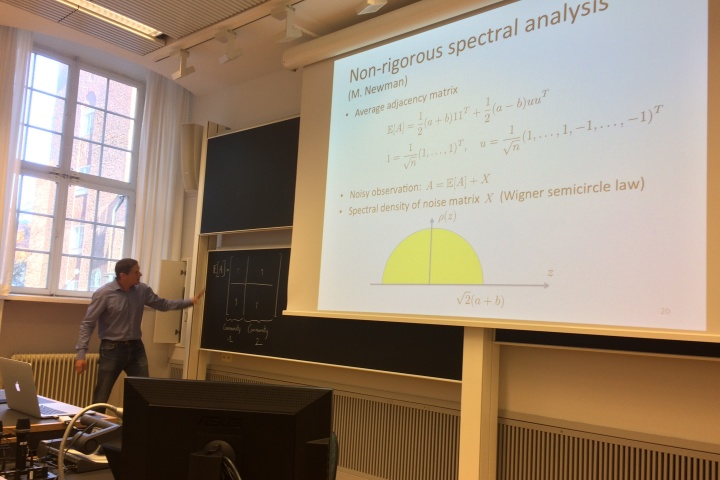
\includegraphics[width=\textwidth]{lecture.jpg}}}
{\fcolorbox{waspgrey}{white}{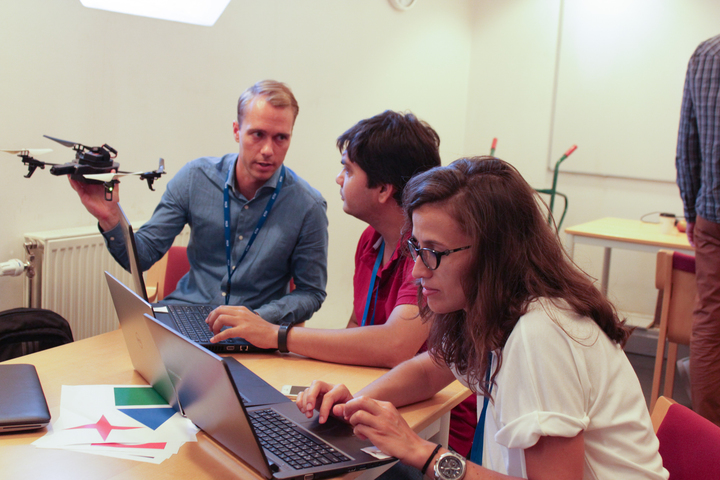
\includegraphics[width=\textwidth]{summerschool.jpg}}}
{\fcolorbox{waspgrey}{white}{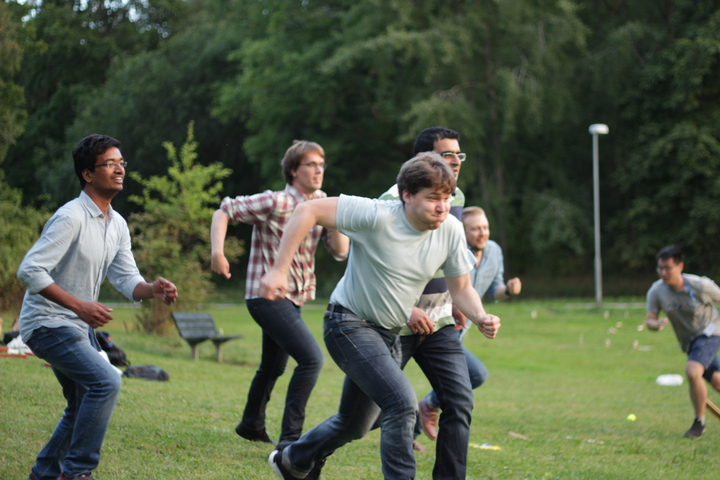
\includegraphics[width=\textwidth]{summer-social.jpg}}}
\end{frame}
\note{Yearly kick-off course with lectures, activities and lots of evening work.}

\begin{frame}
\begin{center}
{\Huge Enjoy!}
\end{center}
\end{frame}

\end{document}
%%% Local Variables:
%%% mode: latex
%%% TeX-master: t
%%% End:
